\documentclass{IEEEtran}
\usepackage{lipsum}
\usepackage{cite,graphicx,amssymb,amsfonts,booktabs,multirow,array,comment}
\usepackage[cmex10]{amsmath}
\usepackage[caption=false,font=footnotesize]{subfig}
\usepackage[all,graph]{xy}
\usepackage{ngerman}
 \usepackage{url}
\usepackage[T1]{fontenc}
\usepackage[utf8]{inputenc}
\title{Starcraft 2 Reinforcement Learning}
\author{\IEEEauthorblockN{Ibrahim Cinar, Tobias Grasmeyer, Artur Schmidt} \\
\IEEEauthorblockA{Fachbereich Informatik\\
Hochschule Darmstadt}
}

\begin{document}
\maketitle
\section{Einführung}
Hier die Aufgabe erklaeren und Starcraft bisschen beschreiben
\section{Starcraft 2 Learning Enviroment}

\section{Q-Learning}
Der Q-Learning Algorithmus gehört zu den Reinforcement Learning Algorithmen und wird hier näher betrachtet. Es enthält eine Tabelle mit einer Liste von Status und eine Liste von Aktionen für jede Status. Der Agent kann für jede  Durchführung einer Aktion eine Belohnung bekommen. Die Werte werden in der Q-Learning Tabelle angepasst. In Bezug zur Starcraft 2 können Aktion z.B. selectArmy (wähle Army aus), attack (angreifen) oder donothing (nichts tun) sein. Status sind z.B. Armeegröße oder ArmySupply.
Beim Start eines Spiels wird eine Q-Learning Tabelle mit den Werten 0 erstellt. Dadurch hat der Agent am Anfang keine Erfahrung. 
Durch die Ausführung einer Aktion der Agent bekommt man eine Belohnung. Dies wird in Form von Werten in einer Q-Learning Tabelle angepasst z.B. falls die Aktion Attack ausgeführt wurde und erfolgreich ist, wird der Wert der Belohnung erhöht. Der Belohnungswert wird in der folgende Formel verwendet:

\[q = reward + \gamma * \max(Q(s',all_a) \]

In dieser Formel ist $reward$ die Belohnungswert. Der Parameter $\gamma$ ist eine Nachlasswert zwischen 0 und 1. Dieser Wert entscheidet, wie wichtig die mögliche nächste Belohnung $\max(Q(s',all_a)$ im Bezug zu den aktuellen Belohnung ist. Wenn der Wert näher zu 0 ist, dann benutzt der Agent den aktuellen Belohnungsfunktion. Falls der Wert auf eins ist, dann  berücksichtigt der Agent den nächsten Belohnungswert mit einer höheren Gewichtung. Diese Formel stellt eine Lernwert dar.
In der folgende Funktion wird der Ergebnis dieser Lernwert, in einer anderen Formel verwendet und in der Q-Learning Tabelle geschrieben.

\[q_t(s, a)= q_t(s, a)+ lr * (q - q_t(s,a) \]

In dieser Formel ist $q_t$ die Q-Learning Tabelle. Der Wert wird in Tabelle von $s$ Status und $a$ Aktion genommen. Diese Wert wird mit Lernfaktor $lr$ mit den Wert 0.9 multipliziert mit den neuen Wert $(q - q_t(s,a)$ addiert. Dadurch wird der Tabelle mit der neuen berechnete Wert aktuell gehalten. Somit wird neue Erfahrung gesammelt. Dies wird in jeder Step des Spiels benutzt. Somit kann man mit Q-Learning Tabelle die Wahrscheinlichkeit sehen, wie gut die Kombination mit Status und Aktion ist \cite{qlearn1} \cite{qlearn2}.

\section{A3C Algorithmus}
Die A3C (Asynchronous Advantage Actor-Critic) Algorithmus wurde von Google's DeepMind 2016 veröffentlicht. Es ist effizienter als die DQN (Deep Q-Network). Der A3C Algorithmus benutzt wie im Figure 1 dargestellt einen neuronalen Netzwerk mit den Wertefunktion $V(s)$, um zu schätzen, wie gut eine bestimmte Status $s$ ist und die Policy Funktion $\pi(s)$, die eine Menge von Aktionen mit Wahrscheinlichkeit ausgibt. Die Agenten benutzen die Wertefunktion, um die Policy aktuell zu halten. Die beiden Funktionen liegen in der Convolutional layer. Die A3C lernt durch die Policy Gradient Methode mit Hilfe von Status $s$. \\
\begin{figure}[!t]
\centering
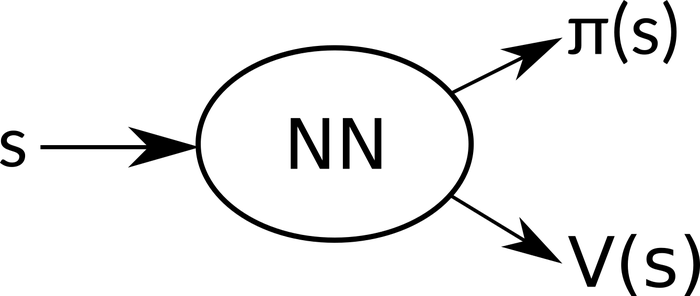
\includegraphics[width=2.5in]{a3c_nn_2.png}
\caption{Neuronale Netzwerk mit der Output von Wertefunktion und Policy Funktion}
\label{fig_sim}
\end{figure}
Der A3C-Algorithmus nutzt mehrere Agenten für mehrere Umgebungen, um effizienter zu lernen. Es hat einen globalen Netzwerk und mehrere Agenten. Jeder dieser Agenten hat eine Menge von Parametern für ihre eigene neuronale Netze und interagieren mit der eigene Umgebung. Der Grund dafür das es effektiver arbeitet als eine einzelne Agent ist, dass die Erfahrungswerte der einzelnen Agenten unabhängig voneinander sind. Die gesamte Verfügbarkeit der Erfahrungswerte für das Lernen der Interaktionen ist sehr vielfältig \cite{A3C1} \cite{A3C2} \cite{A3C3}.

\section{A3C Algorithmus in Starcraft 2}
In Figure 2 sieht man den Ablauf für jeden Agent in A3C. Der Implementierung besteht aus eine AC\_Network, die Funktionen von Tensorflow\footnote{Tensorflow ist eine plattformunabhängige Open-Source-Programmierbibliothek für Künstliche Intelligenz bzw. maschinelles Lernen im Umfeld von Sprache und Bildverarbeitungsaufgaben \cite{Tensor}.} enthalten, um neuronale Netze zu erstellen und Worker, die als Agent erzeugt wird. 
\begin{figure}[!t]
\centering

\includegraphics[width=3.5in]{test.png}
\caption{Durchführung eines Agenten in A3C}
\label{fig_sim}
\end{figure}
Der Algorithmus erstellt eine globale Netzwerk. Diese Netzwerk besteht aus Convolutional Layer, um räumliche Abhängigkeiten abzuarbeiten. Zusätzlich hat es einen Long short-term Memory\footnote{LSTM ist eine spezielle Art von Rekurrentes neuronales Netz. Sie können für längere verzögerte Effekte z.B. für Klassifizierungsaufgaben berücksichtigen und effektiv trainiert werden \cite{LSTM}.} Schicht, um zeitliche Abhängigkeiten abzuarbeiten. Dort sind Werte- und Policyausgabe enthalten.
Beim Erstellen von Agenten wird eine Kopie von globale Netz für die lokale Netz der Agenten erzeugt. Der Agent interagiert mit seine Umgebung und hält die globale Netz in aktuellen Stand. Es wird eine bestimmte Anzahl von Agenten mit eigenen Umgebung und neuronalen Netzen erstellt. In diesem Fall für die Starcraft 2 wird nur eine Agent erstellt. Die Werte der Agenten Parameter wird an den globalen Netze angepasst. Dies geschieht mit Hilfe der Tensorflow. Der Agent hat eine bestimmte Anzahl von Aktionen, die er während der Durchlauf verwenden kann. Für den Beispiel mit der Minimap DefeatRoaches werden 17 Aktionen verwendet. In Worker Agent sind die mögliche Aktionen in einer Methode aufgelistet, die eine Agent machen kann. Jeder Agent interagiert mit seine Umgebung und sammelt somit Erfahrungen.  Dabei gibt es eine Tupel von Erfahrung (Beobachtung, Aktion, Belohnung). Wenn die Historie der Erfahrung groß ist, benutzt man es, um die Ergebnisse und Vorteile zu ermitteln. Diese werden dann mit Value und Policy losses berechnet.
\[Value Loss: L = \sum{(R - V(s))}^2 \]
\[Policy Loss: L = -\log{(\pi(s))} * A(s) -\beta*H(\pi) \]
Die Parameter $R = \gamma(r)$ stellt die reduzierte Belohnung von $r$ dar. Dies wird für ... verwendet. Die Formel $A(s,a) = Q(s,a) - V(s)$ beschreibt wie gut eine Aktion $a$ unter den Status $s$ ist. 
Der Agent benutzt diese Losses Funktionen, um die Gradienten mit Berücksichtugung deren Parameter zu erhalten. 
Der Agent benutzt die Gradient, um die globale Netzwerkparameter zu aktualisieren. Der globale Netzwerk ist somit in einer aktuellen Stand. 
Sobald es aktuell ist, wird der Parameter der Agenten erneuert bzw. resettet und der Prozess startet wieder von neu. 
In der Beispiel werden Schritte (Steps), Episoden, Belohnungswert (Reward), die maximale Punktzahl in der Konsole angezeigt. Somit kann man bei gewissen Anzahl von Durchläufe erkennen, wie der Fortschritt der A3C Algorithmus ist \cite{A3C3}.
\section{Fazit}

\bibliographystyle{IEEEtran}  
\bibliography{Literatur}


\end{document}
